% change this if you want to work in english, or use a different bibliography
% style
%
% For instance, the following would use apa7:
% bibstyle=apa
%
% If your document is in English instead of Dutch, simply remove dutch
% (do not add 'english')
%
% Ex: \documentclass[bibstyle=apa]{adsai}
%
% would make an English document with an apa7-compliant bibliography
%
% Ex: \documentclass[bibstyle=ieee, dutch]{adsai}
%
% would make a Dutch document with an ieee-compliant bibliography
%
% you can mix and match these as you wish.
\documentclass{adsai}

% the title of your project
\title{Activity tracking with the Reachy Mini robot}
% the title of the module, such as 'Design Science Research' or 'Data Science'
\modulename{Artificial Intelligence}

% list of authors
\author{
Caio de Alcantara Santos (1234567890) \\
Cas Limpens (1234567890) \\
Donné Deguelle (1234567890) \\
Gustavo Gonçalves da Costa (1234567890) \\
Kanak Manjari (supervisor) \\
Maarteen Vaessen (supervisor)
}

% academic year that this document is due in
\academicyear{2026/2027}
% the period that this document is due in
\period{Q1}
% the date that this document is due
\date{01-01-2026}

\begin{document}
\maketitle % this adds the title, authors etc. to the beginning of your document

\newpage

\abstract{Home-based exercise monitoring could reduce repeated hospital visits, but it requires reliable activity recognition in unconstrained environments. This project investigates whether the Reachy Mini robot can provide person detection and activity monitoring while giving feedback as an exercise buddy. A feasibility prototype was developed using a camera-to-pose-to-classifier pipeline. The system tracks a person, extracts COCO-17 keypoints, computes temporal features, and classifies activities with random forest inference. The shared pipeline can run both in simulation and on the physical robot. MoveNet int8 was selected for the robot because of its hardware constraints, and recognized actions trigger antenna responses. Evaluation used subject-separated public skeleton datasets, external datasets, recorded robot footage, and both full-body and waist-up framing. In real-time evaluation, wave, clapping, and jumping jacks were sufficiently reliable for demonstration. Overall, the results support the Reachy Mini as a feasible CPU-based platform for activity-monitoring research, while showing that this prototype is not a CMAS scorer or a clinically validated decision-support system.}

\thispagestyle{empty}

\newpage

\section{Introduction}

\subsection{Background}

The Research Centre for Data Intelligence conducts applied research into, among
other themes, smart assistants and human-computer interaction. This project
was carried out in the context of the centre's ``Measuring at Home with AI''
research direction. The long-term motivation for that research is to make
exercise monitoring more accessible to children with juvenile dermatomyositis
(JDM). These children currently perform exercises related to the Childhood
Myositis Assessment Scale (CMAS) under the supervision of specialists at the
Wilhelmina Children's Hospital (WKZ). Repeated travel to the hospital is
burdensome for children and their families, which creates an opportunity for
technologies that can support monitoring at home.

Automated home monitoring must do more than record a video. It must detect a
person, estimate body movement from visual input, distinguish between
activities, and communicate its interpretation clearly to the user. It must
also operate under practical conditions, such as changing distances,
incomplete views of the body, and limited computing resources. The stakeholders
for this feasibility study are the Research Centre for Data Intelligence, the
project client and researcher, and the children and families who represent the
future users of a home-monitoring system. The project requirements were
consolidated in a software requirements specification covering perception,
robot interaction, activity recognition, feedback, session management, privacy,
accuracy, reliability, usability, and safety. The current project addresses the
technical feasibility of such a system; it does not develop or validate a
medical assessment instrument.

\subsection{Opportunity}

A smartphone or tablet could provide a camera for movement monitoring, but a
robot offers an additional interaction layer. The Reachy Mini can follow a
person with its head and body, process camera input on its own computer, and
respond through head and antenna movements. These behaviours make it possible
to present the system as an exercise buddy rather than only as a measurement
device. Such expressive feedback may help make an interaction more
understandable and engaging, particularly for children exercising without a
specialist in the room. Engagement, adherence, and clinical acceptability are
important future questions, but they are outside the evaluation of this
prototype.

\subsection{Goal and scope}

The goal of this project is to investigate whether the Reachy Mini can perform
person detection and activity monitoring, including expressive feedback, under
the computational constraints of the wireless robot. The resulting artefact is
a working prototype that runs in simulation and on the physical robot. It
contains a shared camera-to-pose-to-classifier pipeline, temporal feature
extraction, activity-recognition models, and robot applications that translate
recognized actions into antenna responses. Candidate vision models were
benchmarked under the robot's CPU constraints, leading to the selection of
MoveNet int8 for on-robot pose estimation. Model-training and export tools were
also developed so that the robot can perform inference with NumPy-only model
files rather than requiring the full training environment. Recognition models
were evaluated on public skeleton datasets with subject or footage-group
separation, as well as on robot recordings and an external dataset. Users can
also record personalized movements and create their own datasets for future
recognition models.

The prototype recognizes six classes: none, wave, pushup, squat, clapping,
and jumping jacks. Evaluation focuses on technical feasibility using
simulation, public skeleton datasets, recorded robot footage, an external test
dataset, and different camera framings. The robot's camera should ideally
capture the whole person, because waist-up framing removes information that is
important for some activities.
The prototype is not a CMAS scorer, is not clinically validated, and should
not be used as a clinical decision-support system.

The central research question is:

\begin{quote}
Can the Reachy Mini serve as an engaging, CPU-only platform for home activity
monitoring, and what are the technical and practical limits of the current
prototype?
\end{quote}

The remainder of this article first discusses the theoretical foundations and
related solution space. It then describes the prototype and its evaluation
method, presents the results, discusses their implications and limitations,
and concludes with directions for future development.

\section{Theoretical Framework}

Skeleton-based human activity recognition (HAR) describes a person as a
sequence of body keypoints rather than raw pixels. This reduces each frame to
a few dozen values and makes the input less sensitive to clothing, background
and lighting. The most accurate skeleton classifiers are deep networks. They
lead benchmarks such as NTU RGB+D, but they generally assume GPU hardware. A
lighter, well-established alternative computes hand-crafted statistics over a
sliding temporal window and classifies them with a random forest
\cite{breiman2001random}. This approach is fast, works with modest amounts of
data, keeps its features interpretable and is small enough to run on the device
itself.

Existing work highlights two uncertainties for this approach. First, windowed
activity data contains near-duplicate samples from the same person, so
record-wise train/test splits overestimate performance; subject-wise
validation is needed to approximate the real use case
\cite{saeb2017need}. Second, public datasets are recorded in specific settings,
so a model that scores well on one corpus may not transfer to footage from
another, such as a robot's camera in a living room. The innovative character
of this part of the work is therefore not the classifier itself. It is the
combination of training on published skeleton datasets, evaluating with subject
separation, exporting the forest to a NumPy-only format and connecting it
through the robot's SDK. As a result, recognition runs on the Reachy Mini's CPU
and directly drives expressive feedback.

\section{Methods}

This study employed a custom, iterative methodology to investigate and develop an activity-monitoring system for the Reachy Mini. The approach shares similarities with the Design Science Research (DSR) framework, which is suitable for design-oriented research involving the development and evaluation of an artefact \cite{hevner2007}. The approach was selected because the technical feasibility of the system was initially uncertain and several technical choices required investigation before implementation.

The methodology consisted of five phases:

\begin{enumerate}
    \item Research: identifying stakeholder needs, establishing requirements, and investigating existing techniques.
    \item Design: selecting suitable models and defining the technical architecture.
    \item Realisation: implementing the activity-recognition pipeline and integrating it with the robot.
    \item Testing: evaluating model performance and system behaviour under different conditions.
    \item Evaluation: assessing feasibility, identifying limitations, and formulating recommendations.
\end{enumerate}

The phases were not strictly sequential. Research informed design decisions, while implementation and testing were conducted iteratively. Results from experiments were used to refine technical choices and improve the artefact. This approach supported early validation and incremental improvement, which suited the exploratory nature of the project \cite{geeksforgeeks2025}. A traditional waterfall approach was considered less suitable because the technical choices were not fully determined at the start and the project required opportunities to incorporate findings during implementation \cite{agilescrumgroup}.

Figure~\ref{fig:prototyping-approach} illustrates the iterative prototyping approach. Figure~\ref{fig:research-approach} shows the activities conducted during the research phase.

\begin{figure}[htbp]
    \centering
    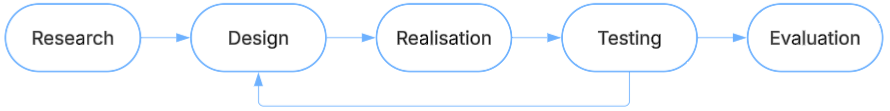
\includegraphics[width=0.9\linewidth]{figures/prototyping-approach.png}
    \caption{Iterative prototyping approach used in the project.}
    \label{fig:prototyping-approach}
\end{figure}

\subsection{Requirements and software requirements specification}

The research began with a stakeholder analysis to identify the parties involved and their interests and needs. Functional and non-functional requirements were derived from the project description and meetings with the client. These requirements were consolidated in a software requirements specification (SRS), which served as the reference for design and evaluation.

The functional requirements cover perception and local processing, robot behaviour and interaction, activity and exercise recognition, assessment and feedback, and session management. The non-functional requirements address privacy, recognition accuracy, reliability, usability, and safety. The complete SRS contains the detailed requirement statements and is included as an attachment to the article.

The research was organised around two complementary activities. First, existing techniques for person detection, pose estimation, and activity recognition were investigated. Second, relevant scientific literature, datasets, standards, and guidelines were studied to identify suitable approaches and relevant constraints. The findings were compared against the system requirements and the Reachy Mini's camera and computational capabilities. This process informed the selection of candidate models and the subsequent evaluation of their suitability.

\begin{figure}[htbp]
    \centering
    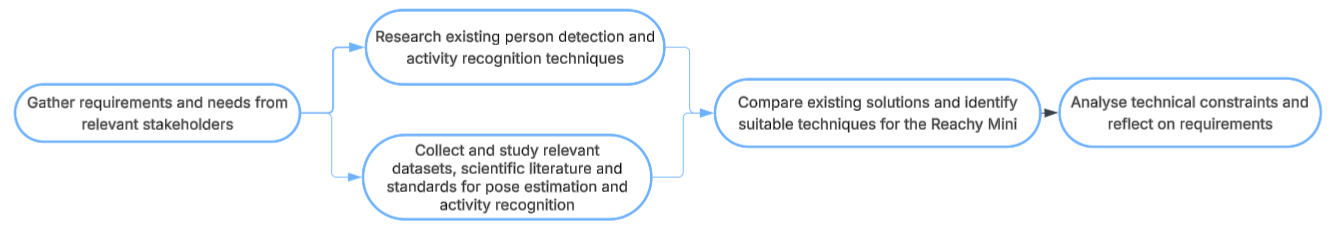
\includegraphics[width=0.9\linewidth]{figures/research-approach.png}
    \caption{Research activities used to establish requirements and identify suitable techniques for the Reachy Mini.}
    \label{fig:research-approach}
\end{figure}

\subsection{Pose-model research and selection}

Candidate models for human pose detection and temporal activity analysis were investigated under the Reachy Mini's CPU and camera constraints. The candidates included BlazePose for fast 2D pose detection, ViTPose as a transformer-based 2D estimator, WHAM and CameraHMR for 3D motion or pose-and-shape estimation, MoveNet for lightweight 2D pose estimation, SAM2 for segmentation, PySlowFast for video classification, FSPose for fused-heatmap pose estimation, GraphEnet for graph-based pose estimation, YOLOPose for pose estimation using the YOLO framework, MoViNets for efficient video recognition, and TSM-MobileNetV2 for lightweight temporal modelling.

BlazePose, MoViNet-A0, TSM-MobileNetV2, ViTPose, YOLOPose, and MoveNet were benchmarked under comparable conditions. Throughput and mean pose-inference time were recorded. The evaluation also considered whether each model could run on the robot and produce the COCO-17 keypoint representation required by the downstream feature-extraction and recognition pipeline.

MoveNet Lightning int8, executed through LiteRT, was selected because it provided the most suitable trade-off between speed, keypoint compatibility, and deployment feasibility.

\subsection{Training, export, and inference}

No new video recordings were collected for model training. Instead, the recognition models were trained using existing COCO-17 skeleton data published by OpenMMLab for NTU RGB+D 60 \cite{shahroudy2016ntu} (wave and clapping) and UCF101 \cite{soomro2012ucf101} (pushup, squat, and jumping jacks). HMDB51 was used only as an external test set. All other dataset classes were labelled as none.

Each clip was resampled from 30 to approximately 10 FPS to match the robot camera. The clips were then divided into temporal windows using the same feature-extraction code as the live system: 1.5-second windows with nine features for the binary wave model, and 3-second windows with 34 features for the six-class action model. To approximate the table-mounted camera perspective, each clip was also windowed with leg and hip keypoints removed.

Random forests were trained using scikit-learn \cite{pedregosa2011scikit}. The wave model used 100 trees with a maximum depth of six, while the action model used 300 class-balanced trees. The models were evaluated using five-fold GroupKFold by subject or footage group, following \cite{saeb2017need}. Precision, recall, and F1 scores were calculated from out-of-fold predictions. A confidence threshold was tuned for each class using these predictions; windows below the threshold were classified as none.

The final forests were fitted on all training windows and exported to compressed \texttt{.npz} files containing the decision-tree node arrays. On the robot, a NumPy-only implementation traverses these trees and reproduces scikit-learn's \texttt{predict\_proba} behaviour, removing the need for scikit-learn during inference.

\subsection{Robot integration}

The applications use the Reachy Mini Python SDK (\texttt{reachy\_mini} 1.10.0, matched to the daemon version) for motion and the daemon REST API on port 8000 for state management.

Before camera, tracking, or movement operations, a standard-library preflight procedure checks network reachability, daemon and backend state, running applications and movements, motor mode, sleep pose, camera ownership, and tracker frames. When automatic correction is enabled, the procedure enables the motors, executes the wake-up movement, and reacquires the camera. It returns an explicit ready, not-ready, or unreachable status. A context manager combines preflight checks, SDK connection, and cleanup, including stopping head tracking and optionally returning the robot to its sleep pose.

Because the vision loop operates at approximately 10 FPS while the daemon controls the robot at 50 Hz, a dedicated thread streams \texttt{set\_target} commands at 50 Hz. Each recognised action produces a distinct antenna movement pattern defined by amplitude, frequency, and a whole number of cycles ending at the neutral pose. Head and body following use an integrating controller based on the image-position error of the torso centre. Body yaw extends the tracking range beyond the head's 60-degree movement limit relative to the body.

Additional integrations include an annotated MJPEG camera stream for browser-based observation without a local display, a remote-inference mode that sends low-resolution frames (192$\times$108 pixels) to a laptop GPU and receives keypoints over HTTP, and a coach workflow for training personalised models on the robot's CPU. In the coach workflow, scikit-learn runs in a low-priority subprocess to keep the camera and tracking loops responsive. A failed training run does not overwrite the previous model. Deployment uses an isolated virtual environment to avoid modifying the robot's system environment.

\subsection{Testing and evaluation}

Testing and evaluation examined the technical feasibility of the system against the requirements established during the research phase. Model performance was assessed using the benchmark results and the out-of-fold precision, recall, and F1 scores. HMDB51 provided an external test set beyond the datasets used for training. Camera-framing experiments considered the effect of removing hip and leg keypoints on the information available for activity recognition.

The evaluation also considered inference speed, CPU-only deployment, compatibility with the Reachy Mini's camera and movement interfaces, and system responsiveness during simultaneous recognition and tracking. The findings were used to identify technical limitations and formulate recommendations for further development. The project focused on technical feasibility; it did not validate a clinical assessment instrument or establish clinical suitability for physiotherapy.

\newpage
\section{Results}

\subsection{Description of the Artefact}
The end product is a software application: a working prototype (an instantiation, in Design Science Research terms) that turns the Reachy Mini into a CPU-only activity monitor that answers what it sees with its own body.
It consists of three parts: a layered software architecture that runs the same recognition code in simulation and on the robot, recognition models exported as NumPy-only files, and robot applications built on both.
It addresses the requirements of the software requirements specification (SRS) attached to this article (Section~3.1).

\begin{figure}[htbp]
  \centering
  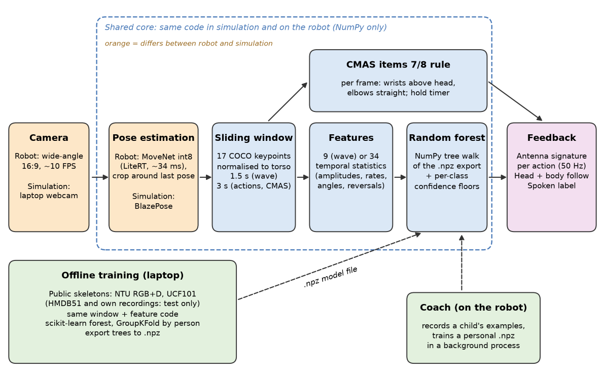
\includegraphics[width=\linewidth]{figures/pipeline_architecture.png}
  \caption{Pipeline Architecture.}
  \label{fig:pipeline}
\end{figure}

Figure~\ref{fig:pipeline} represents the artefact's pipeline.
Everything inside the dashed line is the same code in simulation and on the robot; only the camera and the pose estimator differ.
Models are trained offline, or by the coach on the robot, and loaded as \texttt{.npz} files.

The pipeline works in such way that a camera frame goes to a pose estimator that returns 17 COCO keypoints: MoveNet Lightning int8 on the robot, BlazePose on the laptop webcam in simulation.
The keypoints enter a sliding window, are normalised to the torso and summarised as temporal features.
A random forest, evaluated by a NumPy-only tree walk, classifies every window, and a per-class confidence floor turns uncertain windows into \emph{none}.
Each detection drives the feedback: a distinct antenna signature per action, rendered at 50~Hz independently of the 10~FPS vision loop, head and body following that keeps the person in view, and an optional spoken label.

As for architecture and organization, the code is organised by where it must run: a shared core (pose backends, features, models, feedback), robot applications, simulation tools for MuJoCo and a webcam, and training tools, which are the only part that needs scikit-learn.
Dependencies point only into the core, so one model file and one feature implementation serve both environments, and training and inference cannot drift apart.

For the final application, the robot runs action recognition (the six classes, or the CMAS items of Section~4.6), wave recognition, head and body tracking, and a coach for children.
The coach guides a child through about 4.5 minutes of recording (squats, arm raises, side bends), trains a personal model on the robot's own CPU while the head keeps following, and then runs a workout with that model.
A preflight tool brings the robot into a known state before every application.

Table~\ref{tab:decisions} links the main decisions to the requirement or insight behind them.

\begin{table}[htbp]
  \centering
  \caption{Origin of the main design decisions.}
  \label{tab:decisions}
  \rowcolors{2}{white}{white}
  \begin{tabular}{|p{0.44\textwidth}|p{0.44\textwidth}|}
    \hline
    \rowcolor{gray!20}\textbf{Origin} & \textbf{Decision} \\
    \hline
    Requirement: local processing on a CPU without GPU & MoveNet int8 for pose; forests exported to NumPy instead of a deep skeleton network \\
    \hline
    Requirement: privacy of child users & Only keypoints are stored; children's recordings and models stay on the robot \\
    \hline
    Grounding: windowed data leaks between splits & Every score from GroupKFold by person \\
    \hline
    Grounding: public datasets may not transfer to a room & Robot and room recordings kept as external test sets only \\
    \hline
    Design cycle: BlazePose cannot run on the robot's CPU (its binary needs AES instructions) & Pose backend made swappable behind one interface \\
    \hline
    Design cycle: a table-mounted camera often sees the person waist-up & Training windows also built with hips and legs removed \\
    \hline
    Design cycle: letterboxing the 16:9 wide-angle frame left the person a few dozen pixels tall & Pose crop centred on the previous pose; person detected in 72\% of frames instead of 52\% \\
    \hline
    Design cycle: scikit-learn inference cost ${\sim}33$~ms per window on the robot & Trees exported to \texttt{.npz} and walked in NumPy \\
    \hline
    Design cycle: the robot often boots asleep, motors off, camera released & Preflight with automatic fix \\
    \hline
  \end{tabular}
\end{table}

\subsection{Pose-Model Performance}
The benchmark compared BlazePose, MoViNet-A0, TSM-MobileNetV2, ViTPose and MoveNet as candidates for the perception pipeline.
MoveNet Lightning int8 reached 23.80~FPS in the inference benchmark, with a mean pose-inference time of approximately 34~ms on the Reachy Mini; in the complete application the camera, at about 10~FPS, sets the rate (Section~4.5).
This was the most suitable result for the CPU-only target, and the model produces the COCO-17 keypoints the recognition code expects.
Cropping each frame around the previous pose, instead of letterboxing the whole wide-angle frame, raised the share of robot frames with a detected person from 52\% to 72\%.
On a replay of a laptop recording with the robot's aspect ratio, it raised the mean keypoint confidence from 0.48 to 0.68.

\subsection{CMAS Items}
In CMAS mode the prototype recognises that four CMAS items were performed; it does not score them.
Items~12 (chair rise) and~14 (pick-up) are classified by a three-class forest (none, chair rise, pick-up) trained on NTU RGB+D alone (actions \enquote{standing up} and \enquote{pick up}).
Items~7 and~8 (arms straight above the head, and for how long) use a geometric rule on single frames, because a held posture has no movement for a window to learn.
Item~13 (stool step) was left out: no public dataset contains it and none was recorded.

\section{Discussion}

Several choices contributed positively to the results. Training on skeletons from public datasets gave the project a fast start: working recognition models existed before any data of our own had been recorded, and no video had to be processed. That head start had a limit, however. The public datasets did not cover every exercise the project needed, and they did not show a person the way the robot sees one, so we later had to record our own sessions to train and test the models that mattered most. A second positive choice was to run the same code in simulation and on the robot. Features, models and feedback were developed and checked on a laptop, then deployed to the robot unchanged, which kept the two environments from drifting apart. Finally, short design cycles on the physical robot exposed problems that no laptop test would have shown. They revealed that BlazePose cannot run on the robot's processor, and that letterboxing the wide-angle image left the person too small to detect reliably. Each problem was found and fixed within days, and the crop around the previous pose raised the share of frames with a detected person from 52 percent to 72 percent. \newline

Other aspects limited the results. The robot's camera does not match the image quality of a laptop or phone camera. Its wide-angle view leaves a person only a small part of the image, so keypoints are less certain than in simulation. The CPU, without a GPU, also restricted the choice to a lightweight pose model. A further limit was the difference between the training videos and real use. The public datasets were recorded in studios or taken from films, with other backgrounds, camera angles and sometimes several people in view. The robot, in contrast, sees one person in a home room from table height. This difference lowered recognition quality outside the datasets: waves, for example, scored F1 0.918 on dataset subjects but 0.581 on our robot recordings. The robot was also not always available to the team. The simulation largely mitigated this risk, because most of the development could continue without it. Lastly, engagement could not be measured, because the prototype could not be tested with real users. Whether children find the robot an engaging exercise buddy therefore remains an open question.

\newpage
\section{Conclusion}
The goal was to find out whether the Reachy Mini can detect a person,
recognise their activity and give expressive feedback within the limits
of its own CPU. For the technical part of that goal the answer is
The complete pipeline runs on the robot's Raspberry Pi CM4
without a GPU or a laptop. Pose estimation takes about 34 ms per
frame, features and forest a few milliseconds, and the camera's 10~FPS,
not the computation, sets the pace. The same code and models run in
simulation, so they are developed on a laptop and deployed unchanged.
Recognised actions are answered in real time with antenna signatures and
head and body following.

The answer to ``how well'' is more limited. In live use, wave, clapping
and jumping jacks were reliable enough to demonstrate, and squats were
recognised with about one repetition in seven missed. Push-ups were not.
Scores on public datasets overstate what happens in a room: the
six-class model recognises waves with $F_1 = 0.918$ on dataset subjects
but $F_1 = 0.581$ on our robot recordings. For the CMAS items, pick-up
held up in a room ($F_1 = 0.933$). Chair rise and arms above the head
were recognised live on the robot, but they have not yet been measured
on a correctly performed room recording. The robot's position also
matters: it must see the whole person, and a waist-up view costs
recognition.

The prototype, its models, the training and export tools, and the coach
were realised. A CMAS score, the stool-step item and clinical validation
were not; they were outside the scope. The ``engaging'' part of the
research question was not evaluated, since no user study was done. The
prototype is therefore a research platform: it shows that
monitoring at home with this robot is technically feasible, but it
cannot yet be used to monitor children with JDM.

That said, there are four recommended next steps:
\begin{enumerate}
    \item Record labelled sessions in real rooms through the robot's own
    camera, following the CMAS instructions, and use them as the reference
    for room performance.
    \item Collect data for the classes that lack it: push-ups, clapping
    on robot footage, and the stool step.
    \item Run a small user study with children and families to measure
    engagement, which the research question assumes, but this project did
    not test.
    \item If CMAS scoring becomes the goal, define the scoring criteria
    with the WKZ specialists and validate the system against their scores.
\end{enumerate}

\newpage
\printbibliography % this adds the bibliography to your document

\newpage
\appendix
\appendixpage

\titleformat{\section}{\bfseries\Large}{Appendix \thesection:}{0.5em}{}
\appendix
\section{Software Requirements Specification}

\includepdf[pages=-, scale=0.80, pagecommand={\thispagestyle{plain}}]{appendix/SRS.pdf}


\end{document}
